\subsection{Badania w zakresie najefektywniejszych konfiguracji neuronów}
Biorąc pod uwagę wyniki poprzednich eksperymentów oszacowano zakres neuronów, przy których sieć osiągała najlepsze wyniki. Przeprowadzono kolejne badanie w celu znalezienia najlepszej konfiguracji. Zdecydowano się by badać ilość neuronów w pierwszej warstwie w zakresie od 40 do 80 z krokiem 5 i ilość neuronów w drugiej warstwie od 5 do 30 z krokiem 1.
\begin{figure}[!h]
\centering
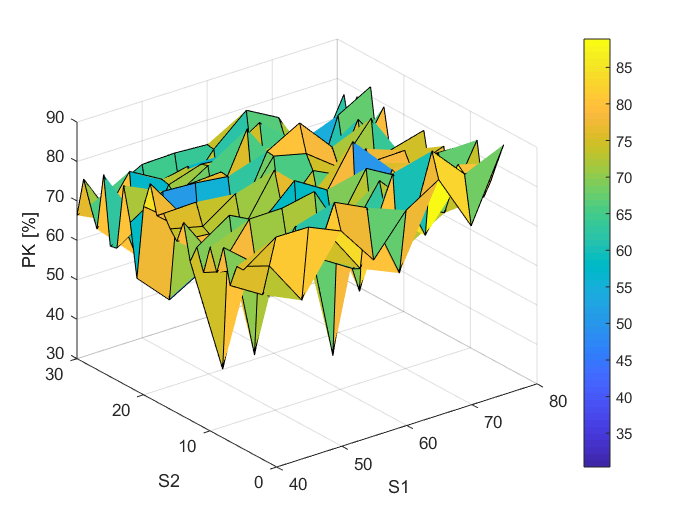
\includegraphics[width = 0.65\textwidth]{Grafika/pk4.png}
\caption{Wpływ liczby neuronów w warstwie pierwszej i drugiej na poprawność klasyfikacji}
\label{fig:PKeksperyment4}
\end{figure}
\begin{figure}[!h]
\centering
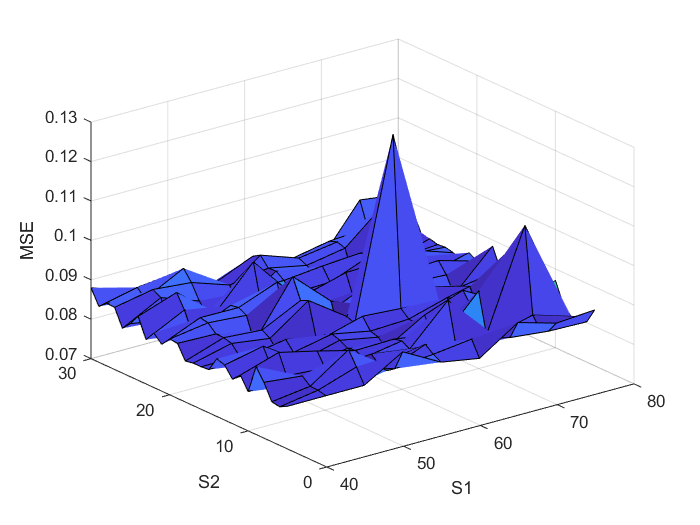
\includegraphics[width = 0.65\textwidth]{Grafika/MSE4.png}
\caption{Wpływ liczby neuronów w warstwie pierwszej i drugiej na błąd średnio-kwadratowy}
\label{fig:MSEeksperyment4}
\end{figure}

Największą poprawność klasyfikacji ($88.88\%$) uzyskano dla 70 neuronów w warstwie pierwszej i 6 w warstwie drugiej. Jednak, kilkukrotnie powtarzając te badanie nie udało się uzyskać podobnego wyniku. Średnio, najlepszą konfiguracją okazało się 70 neuronów w warstwie pierwszej i 13 neuronów w warstwie drugiej dla której większość wyników przekraczała $80\%$ poprawności klasyfikacji.\\
Najmniejszy błąd średnio-kwadratowy ($0.0766883$) osiągnięty został dla 50 neuronów w warstwie pierwszej i 8 neuronów w warstwie drugiej. Dla tej konfiguracji $PK$ wyniosło $72.13\%$.\\